% cpu/overheads.tex

\section{Overheads}
\label{sec:cpu:Overheads}

This section presents actual overheads of the obstacles to performance
listed out in the previous section.
However, it is first necessary to get a rough view of hardware system
architecture, which is the subject of the next section.

\subsection{Hardware System Architecture}
\label{sec:cpu:Hardware System Architecture}

\begin{figure}[tb]
\begin{center}
\resizebox{3in}{!}{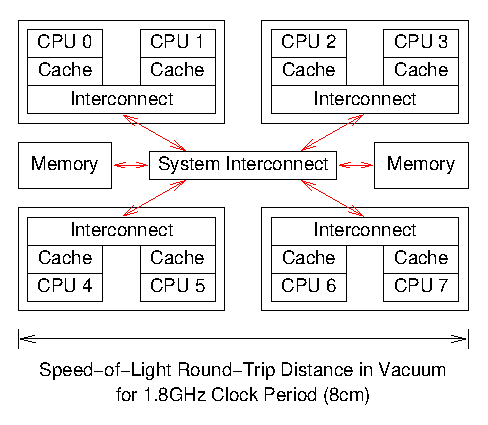
\includegraphics{cpu/SystemArch}}
\end{center}
\caption{System Hardware Architecture}
\label{fig:cpu:System Hardware Architecture}
\end{figure}

Figure~\ref{fig:cpu:System Hardware Architecture}
shows a rough schematic of an eight-core computer system.
Each die has a pair of CPU cores, each with its cache, as well as an
interconnect allowing the pair of CPUs to communicate with each other.
The system interconnect in the middle of the diagram allows the
four dies to communicate, and also connects them to main memory.

Data moves through this system in units of ``cache lines'', which
are power-of-two fixed-size aligned blocks of memory, usually ranging
from 32 to 256 bytes in size.
When a CPU loads a variable from memory to one of its registers, it must
first load the cacheline containing that variable into its cache.
Similarly, when a CPU stores a value from one of its registers into
memory, it must also load the cacheline containing that variable into
its cache, but must also ensure that no other CPU has a copy of that
cacheline.

For example, if CPU~0 were to perform a compare-and-swap (CAS) operation on a
variable whose cacheline resided in CPU~7's cache, the following
over-simplified sequence of events might ensue:

\begin{enumerate}
\item	CPU~0 checks its local cache, and does not find the cacheline.
\item	The request is forwarded to CPU~0's and 1's interconnect,
	which checks CPU~1's local cache, and does not find the cacheline.
\item	The request is forwarded to the system interconnect, which
	checks with the other three dies, learning that the cacheline
	is held by the die containing CPU~6 and 7.
\item	The request is forwarded to CPU~6's and 7's interconnect, which
	checks both CPUs' caches, finding the value in CPU~7's cache.
\item	CPU~7 forwards the cacheline to its interconnect, and also
	flushes the cacheline from its cache.
\item	CPU~6's and 7's interconnect forwards the cacheline to the
	system interconnect.
\item	The system interconnect forwards the cacheline to CPU~0's and 1's
	interconnect.
\item	CPU~0's and 1's interconnect forwards the cacheline to CPU~0's
	cache.
\item	CPU~0 can now perform the CAS operation on the value in its cache.
\end{enumerate}

\QuickQuiz{}
	This is a \emph{simplified} sequence of events?
	How could it \emph{possibly} be any more complex?
\QuickQuizAnswer{
	This sequence ignored a number of possible complications,
	including:

	\begin{enumerate}
	\item	Other CPUs might be concurrently attempting to perform
		CAS operations involving this same cacheline.
	\item	The cacheline might have been replicated read-only in
		several CPUs' caches, in which case, it would need to
		be flushed from their caches.
	\item	CPU~7 might have been operating on the cache line when
		the request for it arrived, in which case CPU~7 might
		need to hold off the request until its own operation
		completed.
	\item	CPU~7 might have ejected the cacheline from its cache
		(for example, in order to make room for other data),
		so that by the time that the request arrived, the
		cacheline was on its way to memory.
	\item	A correctable error might have occurred in the cacheline,
		which would then need to be corrected at some point before
		the data was used.
	\end{enumerate}

	Production-quality cache-coherence mechanisms are extremely
	complicated due to these sorts of considerations.

} \QuickQuizEnd

\QuickQuiz{}
	Why is it necessary to flush the cacheline from CPU~7's cache?
\QuickQuizAnswer{
	If the cacheline was not flushed from CPU~7's cache, then
	CPUs~0 and 7 might have different values for the same set
	of variables in the cacheline.
	This sort of incoherence would greatly complicate parallel
	software, and so hardware architects have been convinced to
	avoid it.
} \QuickQuizEnd

\subsection{Costs of Operations}
\label{sec:cpu:Costs of Operations}

\begin{table}
\centering
\begin{tabular}{l||r|r}
	Operation		& Cost (ns) 	& Ratio \\
	\hline
	\hline
	Clock period		&           0.6	&           1.0 \\
	\hline
	Best-case CAS		&          37.9	&          63.2 \\
	\hline
	Best-case lock		&          65.6	&         109.3\\
	\hline
	Single cache miss	&         139.5	&         232.5 \\
	\hline
	CAS cache miss		&         306.0	&         510.0 \\
	\hline
	Comms Fabric		&       3,000	&       5,000 \\
	\hline
	Global Comms		& 130,000,000	& 216,000,000 \\
\end{tabular}
\caption{Performance of Synchronization Mechanisms on 4-CPU 1.8GHz AMD Opteron 844 System}
\label{tab:cpu:Performance of Synchronization Mechanisms on 4-CPU 1.8GHz AMD Opteron 844 System}
\end{table}

The overheads of some common operations important to parallel programs are
displayed in
Table~\ref{tab:cpu:Performance of Synchronization Mechanisms on 4-CPU 1.8GHz AMD Opteron 844 System}.
This system's clock period rounds to 0.6ns.
Although it is not unusual for modern microprocessors to be able to retire
multiple instructions per clock period, the operations will be normalized
to a full clock period in the third column, labeled ``Ratio''.
The first thing to note about this table is the large values of many of
the ratios.

The best-case CAS operation consumes almost forty
nanoseconds, a duration more than sixty times that of the clock period.
Here, ``best case'' means that the same CPU now performing the CAS operation
on a given variable was the last CPU to operate on this variable, so
that the corresponding cache line is already held in that CPU's cache,
Similarly, the best-case lock operation (a ``round trip'' pair consisting
of a lock acquisition followed by a lock release) consumes more than
sixty nanoseconds, or more than one hundred clock cycles.
Again, ``best case'' means that the data structure representing the
lock is already in the cache belonging to the CPU acquiring and releasing
the lock.
The lock operation is more expensive than CAS because it requires two
atomic operations on the lock data structure.

An operation that misses the cache consumes almost one hundred and forty
nanoseconds, or more than two hundred clock cycles.
A CAS operation, which must look at the old value of the variable as
well as store a new value, consumes over three hundred nanoseconds, or
more than five hundred clock cycles.
Think about this a bit.
In the time required to do \emph{one} CAS operation, the CPU could have
executed more than \emph{five hundred} normal instructions.
This should demonstrate the limitations not only of fine-grained locking,
but of any other synchronization mechanism relying on fine-grained
global agreement.

\QuickQuiz{}
	Surely the hardware designers could be persuaded to improve
	this situation!
	Why have they been content with such abysmal performance
	for these single-instruction operations?
\QuickQuizAnswer{
	The hardware designers \emph{have} been working on this
	problem, and have consulted with no less a luminary than
	the physicist Stephen Hawking.
	Hawking's observation was that the hardware designers have
	two basic problems~\cite{BryanGardiner2007}:

	\begin{enumerate}
	\item	the finite speed of light, and
	\item	the atomic nature of matter.
	\end{enumerate}

\begin{table}
\centering
\begin{tabular}{l||r|r}
	Operation		& Cost (ns) 	& Ratio \\
	\hline
	\hline
	Clock period		&           0.4	&           1.0 \\
	\hline
	``Best-case'' CAS	&          12.2	&          33.8 \\
	\hline
	Best-case lock		&          25.6	&          71.2 \\
	\hline
	Single cache miss	&          12.9	&          35.8 \\
	\hline
	CAS cache miss		&           7.0	&          19.4 \\
	\hline
	Off-Core		&		&		\\
	\hline
	Single cache miss	&          31.2	&          86.6 \\
	\hline
	CAS cache miss		&          31.2	&          86.5 \\
	\hline
	Off-Socket		&		&		\\
	\hline
	Single cache miss	&          92.4	&         256.7 \\
	\hline
	CAS cache miss		&          95.9	&         266.4 \\
	\hline
	Comms Fabric		&       4,500	&       7,500 \\
	\hline
	Global Comms		& 195,000,000	& 324,000,000 \\
\end{tabular}
\caption{Performance of Synchronization Mechanisms on 16-CPU 2.8GHz Intel X5550 (Nehalem) System}
\label{tab:cpu:Performance of Synchronization Mechanisms on 16-CPU 2.8GHz Intel X5550 (Nehalem) System}
\end{table}

	The first problem limits raw speed, and the second limits
	miniaturization, which in turn limits frequency.
	And even this sidesteps the power-consumption issue that
	is currently holding production frequencies to well below
	10 GHz.

	Nevertheless, some progress is being made, as may be seen
	by comparing
	Table~\ref{tab:cpu:Performance of Synchronization Mechanisms on 16-CPU 2.8GHz Intel X5550 (Nehalem) System}
	with
	Table~\ref{tab:cpu:Performance of Synchronization Mechanisms on 4-CPU 1.8GHz AMD Opteron 844 System}
	on
	page~\pageref{tab:cpu:Performance of Synchronization Mechanisms on 4-CPU 1.8GHz AMD Opteron 844 System}.
	Integration of hardware threads in a single core and multiple
	cores on a die have improved latencies greatly, at least within the
	confines of a single core or single die.
	There has been some improvement in overall system latency,
	but only by about a factor of two.
	Unfortunately, neither the speed of light nor the atomic nature
	of matter has changed much in the past few years.

	Section~\ref{sec:cpu:Hardware Free Lunch?}
	looks at what else hardware designers might be
	able to do to ease the plight of parallel programmers.
} \QuickQuizEnd

I/O operations are even more expensive.
A high performance (and expensive!) communications fabric, such as
InfiniBand or any number of proprietary interconnects, has a latency
of roughly three microseconds, during which time five \emph{thousand}
instructions might have been executed.
Standards-based communications networks often require some sort of
protocol processing, which further increases the latency.
Of course, geographic distance also increases latency, with the
theoretical speed-of-light latency around the world coming to
roughly 130 \emph{milliseconds}, or more than 200 million clock
cycles.

\QuickQuiz{}
	These numbers are insanely large!
	How can I possibly get my head around them?
\QuickQuizAnswer{
	Get a roll of toilet paper.
	In the USA, each roll will normally have somewhere around 350-500
	sheets.
	Tear off one sheet to represent a single clock cycle, setting it aside.
	Now unroll the rest of the roll.

	The resulting pile of toilet paper will likely represent a single
	CAS cache miss.

	For the more-expensive inter-system communications latencies,
	use several rolls (or multiple cases) of toilet paper to represent
	the communications latency.

	Important safety tip: make sure to account for the needs of
	those you live with when appropriating toilet paper!
} \QuickQuizEnd
